
\section{图}
	Python代码示例见附录\ref{python_example}，作为附录引用示例。这里是第一个脚注\footnote{第一个脚注示例}，这里是第二个脚注\footnote{第二个脚注示例}
	\subsection{单图示例}
		这是一个单图示例，这个单图的详情见\cref{fig:单图}
		\begin{figure}[htbp]
			\centering
			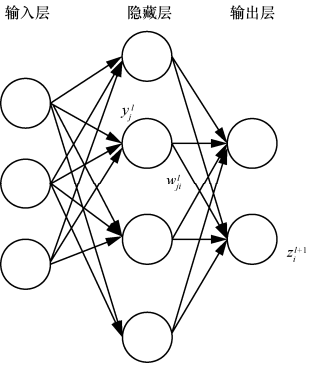
\includegraphics[width = 0.3\textwidth]{./figures/神经网络前向传播.png}
			\caption{这个是单图}
			\label{fig:单图}
		\end{figure}

		上面写了一个单图，接下来写双图

	\subsection{双图示例}

		\subsubsection{两个并列的图}
			\begin{figure}[htbp]
				\centering
				\begin{subfigure}{0.45\textwidth}
					\centering
					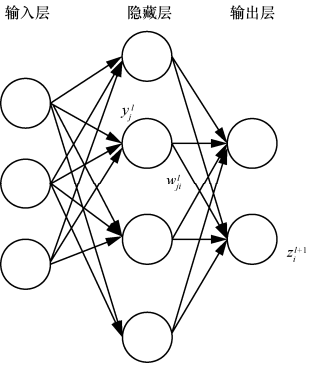
\includegraphics[width = 0.7\textwidth]{./figures/神经网络前向传播.png}
					\caption{这个是双图1}
					\label{fig:双图1}
				\end{subfigure}
				\begin{subfigure}{0.45\textwidth}
					\centering
					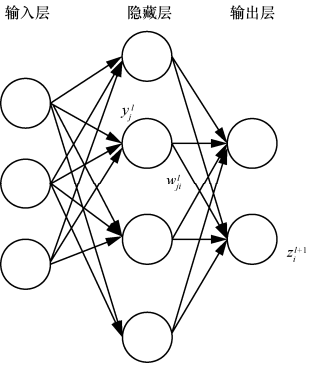
\includegraphics[width = 0.7\textwidth]{./figures/神经网络前向传播.png}
					\caption{这个是双图2}
					\label{fig:双图2}
				\end{subfigure}
				\caption{这里是双图}
			\end{figure}

		双图的引用，可见第一张图：\cref{fig:双图1}，以及第二张图：\cref{fig:双图2}

		\subsubsection{一个图，但是左边有说明}
			\begin{figure}[htbp]
				\centering
				\begin{minipage}[c]{0.45\textwidth}
					\centering
					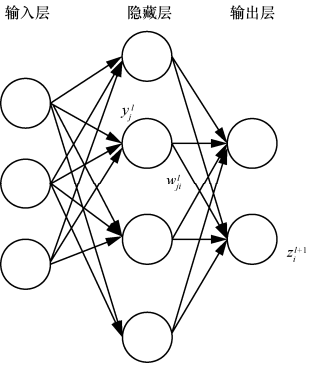
\includegraphics[width=0.7\textwidth]{./figures/神经网络前向传播.png}
					\caption{这是一个有说明的单图}
					\label{fig:说明单图}
				\end{minipage}
				\begin{minipage}[l]{0.45\textwidth}
					 这里是图像说明：这是个神经网络，它有如下特点:

					\begin{itemize}
						\item 有输入层
						\item 有隐藏层
						\item 有输出层
					\end{itemize}

				\end{minipage}
			\end{figure}
		
\newpage


\section{表}
	\subsection{单三线表的示例}
		\begin{table}[htbp]
			\centering
			\caption{不同模型在测试集上的准确率（瞎编版）}
			\label{tab:不同模型的测试结果}
			\begin{tabularx}{\textwidth}{YYYY}
				\toprule
				模型 			& Precision 		& Recall 			& Accuracy \\
				\midrule
				ResNet101 		& 0.91 				& 0.89 				& 0.90 \\
				VGG16     		& 0.88 				& 0.86 				& 0.87 \\
				ViT       		& 0.93 				& 0.92 				& 0.92 \\
				EfficientNet	& 0.92 				& 0.91 				& 0.91 \\
				\textbf{ours}   & \textbf{0.96} 	& \textbf{0.93} 	& \textbf{0.94} \\
				\bottomrule
			\end{tabularx}
		\end{table}

		上面做了三线表的示例，见\cref{tab:不同模型的测试结果}，接下来试试并列双三线表。

	\subsection{双三线表的示例}
		\begin{table}[htbp]
			\centering
			\caption{实验结果（瞎编版）}
			\label{tab:双表示例}
			
			\begin{subtable}[t]{0.45\textwidth}
				\centering
				\caption{消融实验：数据预处理}
				\label{tab:消融实验：数据预处理}
				\begin{tabularx}{0.95\textwidth}{YYY}
					\toprule
					模型 			& Pre Acc  		 	            & Acc \\
					\midrule
					ResNet101 		& 0.90 							& 0.92 \\
					VGG16     		& 0.88 			 				& 0.95 \\
					ViT       		& 0.93 			 				& 0.92 \\
					EfficientNet	& 0.92 			 				& 0.95 \\
					\textbf{ours}   & \textbf{0.93} 			 	& \textbf{0.97} \\
					\bottomrule
				\end{tabularx}
			\end{subtable}
			\hfill   % 注意这里hfill上下不能空行，才能强行将两个表拉成水平
			\begin{subtable}[t]{0.45\textwidth}
				\centering
				\caption{消融实验：数据增强}
				\label{tab:消融实验：数据增强}
				\begin{tabularx}{0.95\textwidth}{YYY}
					\toprule
					模型 			& Pre Acc  		 	            & Acc \\
					\midrule
					ResNet101 		& 0.90 							& 0.92 \\
					VGG16     		& 0.88 			 				& 0.95 \\
					ViT       		& 0.93 			 				& 0.92 \\
					EfficientNet	& 0.92 			 				& 0.95 \\
					\textbf{ours}   & \textbf{0.93} 			 	& \textbf{0.97} \\
					\bottomrule
				\end{tabularx}
			\end{subtable}
		\end{table}

		并列双三线表的示例见\cref{tab:双表示例} ，两个子表分别见\cref{tab:消融实验：数据增强}，以及\cref{tab:消融实验：数据预处理}。

	\subsection{跨页三线表的示例}
		当表格超出一页时，三线表需要用 \texttt{longtable} 环境排版。跨页三线表有两个要求：一是\textbf{表头在每一页重复}，二是\textbf{续页表头要写“表-x 续”，并保留表题说明}，使读者只看续页也能知道该表的内容。跨页三线表的示例如\cref{tab:跨页三线表}。

		\newpage

		\begin{longtable}{@{}c>{\centering\arraybackslash}p{0.26\textwidth}*{4}{>{\centering\arraybackslash}p{0.13\textwidth}}@{}}
			%========== 第一页：表题 + 表头 ==========
			\caption{不同模型在各轮实验中的性能对比（瞎编版，用于演示跨页）}
			\label{tab:跨页三线表}\\
			\toprule
			序号 & 模型 & 参数量/M & Precision & Recall & Accuracy \\
			\midrule
			\endfirsthead

			%========== 续页：重复表头，表题标注“表-x 续”并保留表题说明 ==========
			\multicolumn{6}{c}{\small 表\thetable\ 续\quad 不同模型在各轮实验中的性能对比}\\
			\toprule
			序号 & 模型 & 参数量/M & Precision & Recall & Accuracy \\
			\midrule
			\endhead

			%========== 除末页外，每页底部画线 ==========
			\bottomrule
			\endfoot

			%========== 末页底部画线 ==========
			\bottomrule
			\endlastfoot

			1  & ResNet18        & 11.7   & 0.81 & 0.79 & 0.80 \\
			2  & ResNet50        & 25.6   & 0.84 & 0.83 & 0.83 \\
			3  & ResNet101       & 44.5   & 0.87 & 0.85 & 0.86 \\
			4  & VGG16           & 138.4  & 0.83 & 0.81 & 0.82 \\
			5  & ViT-B/16        & 86.6   & 0.89 & 0.88 & 0.88 \\
			6  & Swin-T          & 28.3   & 0.90 & 0.89 & 0.89 \\
			7  & EfficientNet-B0 & 5.3    & 0.87 & 0.85 & 0.86 \\
			8  & MobileNetV3     & 5.4    & 0.85 & 0.83 & 0.84 \\
			9  & ResNet18        & 11.7   & 0.82 & 0.80 & 0.81 \\
			10 & ResNet50        & 25.6   & 0.85 & 0.84 & 0.84 \\
			11 & ResNet101       & 44.5   & 0.88 & 0.86 & 0.87 \\
			12 & VGG16           & 138.4  & 0.84 & 0.82 & 0.83 \\
			13 & ViT-B/16        & 86.6   & 0.90 & 0.89 & 0.89 \\
			14 & Swin-T          & 28.3   & 0.91 & 0.90 & 0.90 \\
			15 & EfficientNet-B0 & 5.3    & 0.88 & 0.86 & 0.87 \\
			16 & MobileNetV3     & 5.4    & 0.86 & 0.84 & 0.85 \\
			17 & ResNet18        & 11.7   & 0.83 & 0.81 & 0.82 \\
			18 & ResNet50        & 25.6   & 0.86 & 0.85 & 0.85 \\
			19 & ResNet101       & 44.5   & 0.89 & 0.87 & 0.88 \\
			20 & VGG16           & 138.4  & 0.85 & 0.83 & 0.84 \\
			21 & ViT-B/16        & 86.6   & 0.91 & 0.90 & 0.90 \\
			22 & Swin-T          & 28.3   & 0.92 & 0.91 & 0.91 \\
			23 & EfficientNet-B0 & 5.3    & 0.89 & 0.87 & 0.88 \\
			24 & MobileNetV3     & 5.4    & 0.87 & 0.85 & 0.86 \\
			25 & ResNet18        & 11.7   & 0.84 & 0.82 & 0.83 \\
			26 & ResNet50        & 25.6   & 0.87 & 0.86 & 0.86 \\
			27 & ResNet101       & 44.5   & 0.90 & 0.88 & 0.89 \\
			28 & VGG16           & 138.4  & 0.86 & 0.84 & 0.85 \\
			29 & ViT-B/16        & 86.6   & 0.92 & 0.91 & 0.91 \\
			30 & Swin-T          & 28.3   & 0.93 & 0.92 & 0.92 \\
			31 & EfficientNet-B0 & 5.3    & 0.90 & 0.88 & 0.89 \\
			32 & MobileNetV3     & 5.4    & 0.88 & 0.86 & 0.87 \\
			33 & ResNet18        & 11.7   & 0.85 & 0.83 & 0.84 \\
			34 & ResNet50        & 25.6   & 0.88 & 0.87 & 0.87 \\
			35 & ResNet101       & 44.5   & 0.91 & 0.89 & 0.90 \\
			36 & VGG16           & 138.4  & 0.87 & 0.85 & 0.86 \\
			37 & ViT-B/16        & 86.6   & 0.93 & 0.92 & 0.92 \\
			38 & Swin-T          & 28.3   & 0.94 & 0.93 & 0.93 \\
			39 & EfficientNet-B0 & 5.3    & 0.91 & 0.90 & 0.90 \\
			40 & MobileNetV3     & 5.4    & 0.89 & 0.87 & 0.88 \\
			41 & ResNet18        & 11.7   & 0.86 & 0.84 & 0.85 \\
			42 & ResNet50        & 25.6   & 0.89 & 0.88 & 0.88 \\
			43 & ResNet101       & 44.5   & 0.92 & 0.90 & 0.91 \\
			44 & VGG16           & 138.4  & 0.88 & 0.86 & 0.87 \\
			45 & ViT-B/16        & 86.6   & 0.94 & 0.93 & 0.93 \\
			46 & Swin-T          & 28.3   & 0.95 & 0.94 & 0.94 \\
			47 & EfficientNet-B0 & 5.3    & 0.92 & 0.91 & 0.91 \\
			48 & \textbf{Ours}   & \textbf{23.1} & \textbf{0.97} & \textbf{0.95} & \textbf{0.96} \\
		\end{longtable}

		跨页三线表见\cref{tab:跨页三线表}：第一页显示完整表题，表格跨页后，续页顶部会重复表头，并把表题写成“表\ref{tab:跨页三线表} 续\quad 不同模型在各轮实验中的性能对比”的形式（编号自动跟随当前表格，表题说明建议与首页保持一致）。
\newpage

\section{公式}
	\subsection{对齐的长等式}
		
		\begin{align}
			\label{alg:交叉熵损失 }
			\mathcal{L}(\theta)
								&= - \sum_{i=1}^{N} \log p_\theta(y_i \mid x_i)  \nonumber\\
								&= - \sum_{i=1}^{N} \log   \frac{\exp(f_\theta(x_i, y_i))}
											{\sum_{k=1}^{K} \exp(f_\theta(x_i, k))}  \nonumber  \\
								&= - \sum_{i=1}^{N} f_\theta(x_i, y_i)
											+ \sum_{i=1}^{N} \log \sum_{k=1}^{K}
											\exp(f_\theta(x_i, k)) \ .
		\end{align}

	公式示例如\cref{alg:交叉熵损失 }

\newpage

\phantom{ 空一行}
\vspace{-2em}  %修正
\begin{center}
	\zihao{3}\heiti
	\phantomsection
	\addcontentsline{toc}{section}{结\hspace{0.5em}束\hspace{0.5em}语}
	结束语
\end{center}

这里结束语/致谢。可以顺便致谢一下这个模板（doge）。喜欢的学弟学妹别忘了
点个star :)